% Options for packages loaded elsewhere
\PassOptionsToPackage{unicode}{hyperref}
\PassOptionsToPackage{hyphens}{url}
%
\documentclass[
]{article}
\usepackage{lmodern}
\usepackage{amssymb,amsmath}
\usepackage{ifxetex,ifluatex}
\ifnum 0\ifxetex 1\fi\ifluatex 1\fi=0 % if pdftex
  \usepackage[T1]{fontenc}
  \usepackage[utf8]{inputenc}
  \usepackage{textcomp} % provide euro and other symbols
\else % if luatex or xetex
  \usepackage{unicode-math}
  \defaultfontfeatures{Scale=MatchLowercase}
  \defaultfontfeatures[\rmfamily]{Ligatures=TeX,Scale=1}
\fi
% Use upquote if available, for straight quotes in verbatim environments
\IfFileExists{upquote.sty}{\usepackage{upquote}}{}
\IfFileExists{microtype.sty}{% use microtype if available
  \usepackage[]{microtype}
  \UseMicrotypeSet[protrusion]{basicmath} % disable protrusion for tt fonts
}{}
\makeatletter
\@ifundefined{KOMAClassName}{% if non-KOMA class
  \IfFileExists{parskip.sty}{%
    \usepackage{parskip}
  }{% else
    \setlength{\parindent}{0pt}
    \setlength{\parskip}{6pt plus 2pt minus 1pt}}
}{% if KOMA class
  \KOMAoptions{parskip=half}}
\makeatother
\usepackage{xcolor}
\IfFileExists{xurl.sty}{\usepackage{xurl}}{} % add URL line breaks if available
\IfFileExists{bookmark.sty}{\usepackage{bookmark}}{\usepackage{hyperref}}
\hypersetup{
  hidelinks,
  pdfcreator={LaTeX via pandoc}}
\urlstyle{same} % disable monospaced font for URLs
\usepackage{color}
\usepackage{fancyvrb}
\newcommand{\VerbBar}{|}
\newcommand{\VERB}{\Verb[commandchars=\\\{\}]}
\DefineVerbatimEnvironment{Highlighting}{Verbatim}{commandchars=\\\{\},fontsize=\small}
% Add ',fontsize=\small' for more characters per line
\newenvironment{Shaded}{}{}
\newcommand{\AlertTok}[1]{\textcolor[rgb]{1.00,0.00,0.00}{\textbf{#1}}}
\newcommand{\AnnotationTok}[1]{\textcolor[rgb]{0.38,0.63,0.69}{\textbf{\textit{#1}}}}
\newcommand{\AttributeTok}[1]{\textcolor[rgb]{0.49,0.56,0.16}{#1}}
\newcommand{\BaseNTok}[1]{\textcolor[rgb]{0.25,0.63,0.44}{#1}}
\newcommand{\BuiltInTok}[1]{#1}
\newcommand{\CharTok}[1]{\textcolor[rgb]{0.25,0.44,0.63}{#1}}
\newcommand{\CommentTok}[1]{\textcolor[rgb]{0.38,0.63,0.69}{\textit{#1}}}
\newcommand{\CommentVarTok}[1]{\textcolor[rgb]{0.38,0.63,0.69}{\textbf{\textit{#1}}}}
\newcommand{\ConstantTok}[1]{\textcolor[rgb]{0.53,0.00,0.00}{#1}}
\newcommand{\ControlFlowTok}[1]{\textcolor[rgb]{0.00,0.44,0.13}{\textbf{#1}}}
\newcommand{\DataTypeTok}[1]{\textcolor[rgb]{0.56,0.13,0.00}{#1}}
\newcommand{\DecValTok}[1]{\textcolor[rgb]{0.25,0.63,0.44}{#1}}
\newcommand{\DocumentationTok}[1]{\textcolor[rgb]{0.73,0.13,0.13}{\textit{#1}}}
\newcommand{\ErrorTok}[1]{\textcolor[rgb]{1.00,0.00,0.00}{\textbf{#1}}}
\newcommand{\ExtensionTok}[1]{#1}
\newcommand{\FloatTok}[1]{\textcolor[rgb]{0.25,0.63,0.44}{#1}}
\newcommand{\FunctionTok}[1]{\textcolor[rgb]{0.02,0.16,0.49}{#1}}
\newcommand{\ImportTok}[1]{#1}
\newcommand{\InformationTok}[1]{\textcolor[rgb]{0.38,0.63,0.69}{\textbf{\textit{#1}}}}
\newcommand{\KeywordTok}[1]{\textcolor[rgb]{0.00,0.44,0.13}{\textbf{#1}}}
\newcommand{\NormalTok}[1]{#1}
\newcommand{\OperatorTok}[1]{\textcolor[rgb]{0.40,0.40,0.40}{#1}}
\newcommand{\OtherTok}[1]{\textcolor[rgb]{0.00,0.44,0.13}{#1}}
\newcommand{\PreprocessorTok}[1]{\textcolor[rgb]{0.74,0.48,0.00}{#1}}
\newcommand{\RegionMarkerTok}[1]{#1}
\newcommand{\SpecialCharTok}[1]{\textcolor[rgb]{0.25,0.44,0.63}{#1}}
\newcommand{\SpecialStringTok}[1]{\textcolor[rgb]{0.73,0.40,0.53}{#1}}
\newcommand{\StringTok}[1]{\textcolor[rgb]{0.25,0.44,0.63}{#1}}
\newcommand{\VariableTok}[1]{\textcolor[rgb]{0.10,0.09,0.49}{#1}}
\newcommand{\VerbatimStringTok}[1]{\textcolor[rgb]{0.25,0.44,0.63}{#1}}
\newcommand{\WarningTok}[1]{\textcolor[rgb]{0.38,0.63,0.69}{\textbf{\textit{#1}}}}
\usepackage{graphicx}
\makeatletter
\def\maxwidth{\ifdim\Gin@nat@width>\linewidth\linewidth\else\Gin@nat@width\fi}
\def\maxheight{\ifdim\Gin@nat@height>\textheight\textheight\else\Gin@nat@height\fi}
\makeatother
% Scale images if necessary, so that they will not overflow the page
% margins by default, and it is still possible to overwrite the defaults
% using explicit options in \includegraphics[width, height, ...]{}
\setkeys{Gin}{width=\maxwidth,height=\maxheight,keepaspectratio}
% Set default figure placement to htbp
\makeatletter
\def\fps@figure{htbp}
\makeatother
\setlength{\emergencystretch}{3em} % prevent overfull lines
\providecommand{\tightlist}{%
  \setlength{\itemsep}{0pt}\setlength{\parskip}{0pt}}
\setcounter{secnumdepth}{-\maxdimen} % remove section numbering

\author{}
\date{}

% manual margin -- starts here --- 
\addtolength{\oddsidemargin}{-.41in}
\addtolength{\evensidemargin}{-.41in}
\addtolength{\textwidth}{0.82in}

\addtolength{\topmargin}{-.55in}
\addtolength{\textheight}{1.10in}
% manual margin --ends here --

\begin{document}

\hypertarget{topological-sorting}{%
\section{Topological Sorting}\label{topological-sorting}}

\textbf{Topological Sorting} for a Directed Acyclic Graph (\emph{DAG})
is a linear ordering of vertices, such that for every edge from vertex
\emph{u} to \emph{v}, \emph{u} comes before \emph{v}. It is a graph
traversal in which every vertex \emph{a} is visited only after all its
dependencies are visited. For example, topological sorting may be used
to represent an order of tasks to be performed, if every vertex
represents a task and the edges represent a constraint that one task
must be performed before another.

\hypertarget{using-dfs}{%
\subsection{Using DFS:}\label{using-dfs}}

DFS is somewhat modified to get a topological ordering of the vertices.
This algorithm is started from a vertex and then the method is
recursively called for all its adjacent vertices. A temporary stack is
used. For a vertex, after all its adjacent vertices, only then, it is
pushed in the stack. Later, the stack is emptied by popping the vertices
one by one, which is, ultimately, the topological sorting of the DAG.
Consider an edge \(uv\) directed from \(u\) to \(v\). If the vertex
\(v\) occurs before \(u\) in the topological ordering, the graph is not
an DAG.

Below is a implementation of the same in \texttt{topoSortUsingDFS.cpp}.
It uses the \texttt{class\ Graph} as a graph from \texttt{graph.hpp}
mentioned before.

\begin{Shaded}
\begin{Highlighting}[]
\CommentTok{// topoSortUsingDFS.cpp}

\PreprocessorTok{\#include }\ImportTok{"graph.hpp"}

\CommentTok{/**}
\CommentTok{ * }\AnnotationTok{@brief}\CommentTok{ Helps topologicalSort by recursively applying DFS. Reversed topological ordering }
\CommentTok{ * is stored in order.}
\CommentTok{ *}
\CommentTok{ * }\AnnotationTok{@param}\CommentTok{ }\CommentVarTok{G}\CommentTok{ The Graph Object.}
\CommentTok{ * }\AnnotationTok{@param}\CommentTok{ }\CommentVarTok{u}\CommentTok{ The vertex on which DFS is to be performed.}
\CommentTok{ * }\AnnotationTok{@param}\CommentTok{ }\CommentVarTok{order}\CommentTok{ The vector container in which reverse topological ordering is stored.}
\CommentTok{ * }\AnnotationTok{@param}\CommentTok{ }\CommentVarTok{visited}\CommentTok{ The vector boolean container to keep track of visited vertices.}
\CommentTok{ */}
\DataTypeTok{void} 
\NormalTok{topoSortUtil(}\AttributeTok{const}\NormalTok{ Graph \&G, Vertex u, }\BuiltInTok{std::}\NormalTok{vector\textless{}Vertex\textgreater{} \&order, }\BuiltInTok{std::}\NormalTok{vector\textless{}}\DataTypeTok{bool}\NormalTok{\textgreater{} \&visited) \{}
\NormalTok{    visited[u] = }\KeywordTok{true}\NormalTok{;}
    \AttributeTok{const} \BuiltInTok{std::}\NormalTok{vector\textless{}Vertex\textgreater{} \& adj = G.getAdj(u);}
    \ControlFlowTok{for}\NormalTok{ (Vertex v : adj) \{}
        \ControlFlowTok{if}\NormalTok{ (}\KeywordTok{not}\NormalTok{ visited[v]) }
\NormalTok{            topoSortUtil(G, v, order, visited);}
\NormalTok{    \}}
\NormalTok{    order.push\_back(u);}
\NormalTok{\}}


\CommentTok{/**}
\CommentTok{ * }\AnnotationTok{@brief}\CommentTok{ Prints a topological ordering of the vertices if the Graph }
\CommentTok{ * is an DAG. Prints an error message if the Graph is not an DAG.}
\CommentTok{ * }
\CommentTok{ * }\AnnotationTok{@param}\CommentTok{ }\CommentVarTok{G}\CommentTok{ The Graph object}
\CommentTok{ * }\AnnotationTok{@param}\CommentTok{ }\CommentVarTok{err}\CommentTok{ Default = "IMPOSSIBLE". The error message to be prited}
\CommentTok{ * if the graph is not an DAG.}
\CommentTok{ */}
\DataTypeTok{void} 
\NormalTok{topologicalSort(}\AttributeTok{const}\NormalTok{ Graph \&G, }\BuiltInTok{std::}\NormalTok{string err = }\StringTok{"IMPOSSIBLE"}\NormalTok{) \{}
    \DataTypeTok{int}\NormalTok{ V = G.getV();}
    \DataTypeTok{int}\NormalTok{ pos[V + }\DecValTok{1}\NormalTok{]=\{\};}
    \BuiltInTok{std::}\NormalTok{vector\textless{}Vertex\textgreater{} topologicalOrdering;}
\NormalTok{    topologicalOrdering.reserve(V);}
    \BuiltInTok{std::}\NormalTok{vector\textless{}}\DataTypeTok{bool}\NormalTok{\textgreater{} visited(V + }\DecValTok{1}\NormalTok{);}

    \ControlFlowTok{for}\NormalTok{ (Vertex i = Vertex(}\DecValTok{1}\NormalTok{); i \textless{}= V; ++i) \{}
        \ControlFlowTok{if}\NormalTok{ (}\KeywordTok{not}\NormalTok{ visited[i]) }
\NormalTok{            topoSortUtil(G, i, topologicalOrdering, visited);}
\NormalTok{    \}}

    \BuiltInTok{std::}\NormalTok{reverse(topologicalOrdering.begin(), topologicalOrdering.end());}

    \DataTypeTok{int}\NormalTok{ p = }\DecValTok{0}\NormalTok{;}
    \ControlFlowTok{for}\NormalTok{ (Vertex u : topologicalOrdering) \{}
\NormalTok{        pos[u] = p; ++p;}
\NormalTok{    \}}

    \ControlFlowTok{for}\NormalTok{ (Vertex i = Vertex(}\DecValTok{1}\NormalTok{); i \textless{}= V; ++i) \{}
        \AttributeTok{const} \BuiltInTok{std::}\NormalTok{vector\textless{}Vertex\textgreater{} \&adj = G.getAdj(i);}
        \ControlFlowTok{for}\NormalTok{ (Vertex v : adj) \{}
            \ControlFlowTok{if}\NormalTok{ (pos[v] \textless{} pos[i]) \{}
                \BuiltInTok{std::}\NormalTok{cout \textless{}\textless{} err \textless{}\textless{} }\StringTok{"}\SpecialCharTok{\textbackslash{}n}\StringTok{"}\NormalTok{;}
                \ControlFlowTok{return}\NormalTok{; }
\NormalTok{            \}}
\NormalTok{        \}}
\NormalTok{    \}}

    \ControlFlowTok{for}\NormalTok{ (}\DataTypeTok{int}\NormalTok{ u : topologicalOrdering) \{}
        \BuiltInTok{std::}\NormalTok{cout \textless{}\textless{} u \textless{}\textless{} }\CharTok{\textquotesingle{} \textquotesingle{}}\NormalTok{;}
\NormalTok{    \}}
    \BuiltInTok{std::}\NormalTok{cout \textless{}\textless{} }\StringTok{"}\SpecialCharTok{\textbackslash{}n}\StringTok{"}\NormalTok{;}
\NormalTok{\}}
\end{Highlighting}
\end{Shaded}

\begin{Shaded}
\begin{Highlighting}[]
\PreprocessorTok{\#include }\ImportTok{"graph.hpp"}

\DataTypeTok{void}\NormalTok{ topologicalSort(}\AttributeTok{const}\NormalTok{ Graph \&G, }\BuiltInTok{std::}\NormalTok{string err = }\StringTok{"IMPOSSIBLE"}\NormalTok{);}

\DataTypeTok{int}\NormalTok{ main() \{}
\NormalTok{    Graph G(}\DecValTok{6}\NormalTok{, }\KeywordTok{true}\NormalTok{);}
\NormalTok{    G.addEdge(}\DecValTok{1}\NormalTok{, }\DecValTok{2}\NormalTok{);}
\NormalTok{    G.addEdge(}\DecValTok{1}\NormalTok{, }\DecValTok{3}\NormalTok{);}
\NormalTok{    G.addEdge(}\DecValTok{2}\NormalTok{, }\DecValTok{4}\NormalTok{);}
\NormalTok{    G.addEdge(}\DecValTok{2}\NormalTok{, }\DecValTok{5}\NormalTok{);}
\NormalTok{    G.addEdge(}\DecValTok{3}\NormalTok{, }\DecValTok{4}\NormalTok{);}
\NormalTok{    G.addEdge(}\DecValTok{3}\NormalTok{, }\DecValTok{6}\NormalTok{);}
\NormalTok{    G.addEdge(}\DecValTok{4}\NormalTok{, }\DecValTok{5}\NormalTok{);}
\NormalTok{    G.addEdge(}\DecValTok{4}\NormalTok{, }\DecValTok{6}\NormalTok{);}
\NormalTok{    topologicalSort(G);}
    \ControlFlowTok{return} \DecValTok{0}\NormalTok{;}
\NormalTok{\}}
\end{Highlighting}
\end{Shaded}

The example graph used in the \texttt{main.cpp} file is:

\begin{figure}
\centering
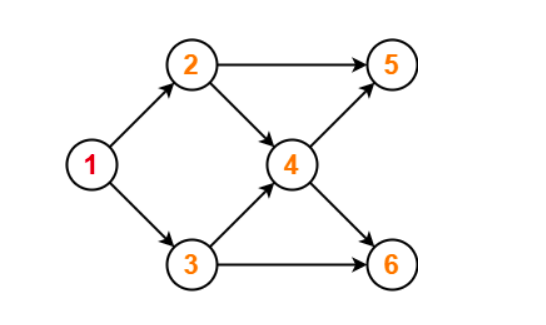
\includegraphics{../mds/eg.png}
\caption{}
\end{figure}

After compiling and running,

\begin{verbatim}
$ g++ topoSortUsingDFS.cpp main.cpp -std=gnu++17 
$ ./a.out
1 3 2 4 6 5 
\end{verbatim}

\begin{itemize}
\item
  Time Complexity: \(O(V+E)\)
\item
  Space Complexity: \(O(V)\)
\end{itemize}

Since this algorithm is a modification of the DFS algorithm with an
extra temporary stack, the time complexity is the same. It needs extra
space for the stack.

\hypertarget{kahns-algorithm}{%
\subsection{\texorpdfstring{Kahn's Algorithm:
}{Kahn's Algorithm: }}\label{kahns-algorithm}}

Kahn's algorithm is based on including vertices with no incoming edges
and eliminating vertices with no outgoing edges.

In this algorithm, a queue is maintained. Initially, the queue is empty.
Also, a count of in-degree of all vertices is maintained. For every
outgoing edge, the in-degree of the destination vertex is incremented.

Then, all vertices with no incoming edge or with in-degree equal to 0 is
enqueued. Then, until the queue is not empty, following steps are
performed:

\begin{itemize}
\item
  A vertex from the queue is dequeued.
\item
  For every such vertex, the in-degrees' of its adjacent vertices are
  decremented.
\item
  After decrementing, if the in-degree becomes equal to 0, the adjacent
  vertex is enqueued in the queue.
\end{itemize}

Below is a implementation of the same in \texttt{topoSortUsingKahn.cpp}.
It uses the \texttt{class\ Graph} as a parameter from \texttt{graph.hpp}
mentioned before.

\begin{Shaded}
\begin{Highlighting}[]
\CommentTok{// topoSortUsingKahn.cpp}

\PreprocessorTok{\#include }\ImportTok{"graph.hpp"}\PreprocessorTok{ }

\DataTypeTok{void}
\NormalTok{topologicalSort(}\AttributeTok{const}\NormalTok{ Graph \&G, }\AttributeTok{const} \BuiltInTok{std::}\NormalTok{string err = }\StringTok{"IMPOSSIBLE"}\NormalTok{) \{}
    \DataTypeTok{int}\NormalTok{ V = G.getV();}
\NormalTok{    Vertex inDegree[V + }\DecValTok{1}\NormalTok{]=\{\};}
    \BuiltInTok{std::}\NormalTok{queue\textless{}Vertex\textgreater{} Q;}
    \BuiltInTok{std::}\NormalTok{vector\textless{}Vertex\textgreater{} topologicalOrdering;}
\NormalTok{    topologicalOrdering.reserve(V);}

    \CommentTok{// Count incoming edges for all vertices}
    \ControlFlowTok{for}\NormalTok{ (Vertex u = Vertex(}\DecValTok{1}\NormalTok{); u \textless{}= V; ++u) \{}
        \AttributeTok{const} \BuiltInTok{std::}\NormalTok{vector\textless{}Vertex\textgreater{} \& adj = G.getAdj(u);}
        \ControlFlowTok{for}\NormalTok{ (Vertex v : adj) \{}
\NormalTok{            inDegree[v]++;}
\NormalTok{        \}}
\NormalTok{    \}}

    \ControlFlowTok{for}\NormalTok{ (Vertex u = Vertex(}\DecValTok{1}\NormalTok{); u \textless{}= V; ++u) \{}
        \CommentTok{// Enqueue the vertex with 0 in{-}degree}
        \ControlFlowTok{if}\NormalTok{ (inDegree[u] == }\DecValTok{0}\NormalTok{) }
\NormalTok{            Q.push(u);          }
\NormalTok{    \}}

    \ControlFlowTok{while}\NormalTok{ (}\KeywordTok{not}\NormalTok{ Q.empty()) \{}
\NormalTok{        Vertex u = Q.front();}
\NormalTok{        Q.pop();}

\NormalTok{        topologicalOrdering.push\_back(u);}

        \AttributeTok{const} \BuiltInTok{std::}\NormalTok{vector\textless{}Vertex\textgreater{} \& adj = G.getAdj(u);}
        \ControlFlowTok{for}\NormalTok{ (Vertex v : adj) \{}

            \CommentTok{// Decrement in{-}degree of adjacent vertex}
\NormalTok{            {-}{-}inDegree[v];}

            \CommentTok{// Enqueue the vertex with 0 in{-}degree}
            \ControlFlowTok{if}\NormalTok{ (inDegree[v] == }\DecValTok{0}\NormalTok{) }
\NormalTok{                Q.push(v);          }
\NormalTok{        \}}
\NormalTok{    \}}

    \ControlFlowTok{if}\NormalTok{ (Vertex(topologicalOrdering.size()) != V) \{}
        \BuiltInTok{std::}\NormalTok{cout \textless{}\textless{} err \textless{}\textless{} }\StringTok{"}\SpecialCharTok{\textbackslash{}n}\StringTok{"}\NormalTok{;}
        \ControlFlowTok{return}\NormalTok{;}
\NormalTok{    \}}

    \ControlFlowTok{for}\NormalTok{ (}\DataTypeTok{int}\NormalTok{ u : topologicalOrdering) \{}
        \BuiltInTok{std::}\NormalTok{cout \textless{}\textless{} u \textless{}\textless{} }\CharTok{\textquotesingle{} \textquotesingle{}}\NormalTok{;}
\NormalTok{    \}}
    \BuiltInTok{std::}\NormalTok{cout \textless{}\textless{} }\StringTok{"}\SpecialCharTok{\textbackslash{}n}\StringTok{"}\NormalTok{;}
\NormalTok{\}}
\end{Highlighting}
\end{Shaded}

The same \texttt{main.cpp} is used and the same example diagram shown
before in the section \emph{Using DFS} of \emph{Topological Sort}.

After compiling and running \texttt{main.cpp},

\begin{verbatim}
$ g++ topoSortUsingKahn.cpp main.cpp -std=gnu++17 
$ ./a.out
1 2 3 4 5 6 
\end{verbatim}

\begin{itemize}
\item
  Time Complexity: \(O(V+E)\)
\item
  Space Complexity: \(O(V)\)
\end{itemize}

\end{document}
